\paragraph{Co zrobiono} Na 1. laboratorium do wzorca dodano 2 funkcje: \funkcja{rufa} oraz \funkcja{kadlub}, stanowiące dno pokładu i kształt jachtu. Kadłub jest po prawej stronie i jest trójkątna, zaś rufa z tyłu i ma kształt graniastosłupa o podstawie będącej trapezem. 
Globalny środek układu współrzędnych wybrano na dnie jachtu, na jego środku, aby ułatwić orientację pozostałych punktów w przestrzeni oraz późniejsze skalowanie. Bowiem jacht można w przybliżeniu uważać za symetryczny wzgl. środka dna.

Tam gdzie kadłub lub rufa łączy się z wnętrzem, wierzchołki są zdublowane. Zdublowane są także dwie ściany.

Dla ułatwienia pisania, stworzono 2 uniwersalne funkcje: \funkcja{drawCuboid} i \funkcja{drawTriangle}. Za ich pomocą stworzono maszt i 2 żagle. Korzystając z mapy miejsca\footnote{wybrano marinę w Turcji, o współrzędnych geograficznych  \ang{36;49;05}N \ang{28;18;32}E}, utworzono linię brzegową, która odgradza również namalowane: \funkcja{akwen} i ląd. 

Początkowo układ współrzędnych był położony ,,po kartezjańsku", tzn. w płaszczyźnie rysunku zawarte były osie x i y, zaś z przecinała płaszczyznę. Uznano, że sprawia to problemy w projektowaniu i komplikuje rozłożenie obiektów. Zmieniono więc orientację tak, że oś z jest pionowa. Dodano również nowe features w zakresie samego okna: standardowe położenie na ekranie, tytuł oraz możliwość poruszania się za pomocą klawiszy numerycznych 2,4,6,8.

\begin{figure}[b]
	Wygląd yachtu przedstawia poniższy rysunek.
	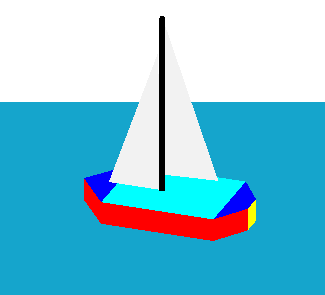
\includegraphics{img/firstBoat}
\end{figure}

Wyznaczony tor ruchu yachtu dla animacji jest pokazany na \autoref{tor}. Jest to linia krzywa, zaczynająca się w punkcie (0. 0) i kończy w (2000, 800). Pierwsza część jest linią prostą, druga łukiem okręgu o promieniu 400.
\begin{figure}[b]
	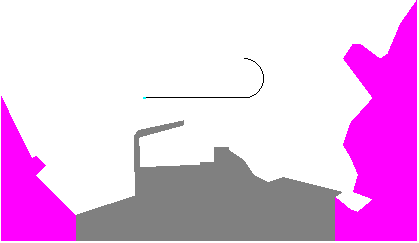
\includegraphics{img/swimmingLine}
	\caption{Tor yachtu w animacji}
	\label{tor}
\end{figure}

Zaprojektowano, zob. rys. \autoref{design}.
\begin{figure}
	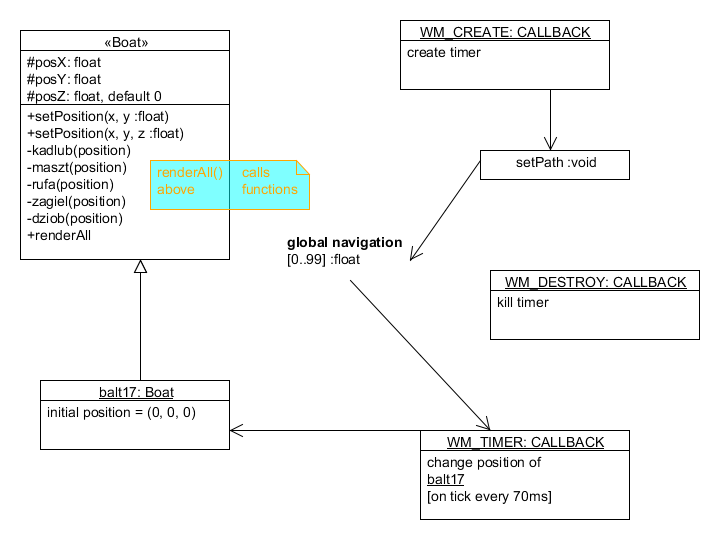
\includegraphics[scale=0.75]{img/yacht}
	\label{design}
\end{figure}

\paragraph{Problemy}
Nastąpiły problemy związane z orientacją osi oraz nazewnictwem punktów \textsc{sa}--\textsc{sh}. Nie było wiadomo, który punkt w kodzie programu odpowiada któremu puntowi na renderze. Nastąpiło kilka pomyłek. Pozostaje niewyjaśnione, dlaczego oś \textit{y} jest pionowa w płaszczyźnie rysunku, zaś oś \textit{z} prostopadła do tej płaszczyzny. 
Następnie stracono dużo czasu z powodu niewłaściwego sposobu wykreowania rufy za pomocą istniejącego kadłuba. Skopiowano początkowo punkty, a następnie zamieniono wartości na osiach \textit{x} oraz \textit{z} na przeciwne. Doprowadziło to do całkowitej dezorientacji, ponieważ punkt \textsc{sa} nie odpowiadał puntowi \textsc{ra}, \textsc{sd} punktowi \textsc{rd} itd.

\paragraph{Wnioski}
Należy trzymać się konsekwentnego nazewnictwa punktów, a w przypadku całkiem nowego punktu, używać unikatowej nazwy.